%%%%%%%%%%%%%%%%%%%%%%%%%%%%%%%%%%%%%%%%%%%%%%%%%%%%%%%%%%%%%%%%%%%%%%%%%%%%%%%%%%%%%%%%%%%%%%%%%%%%%%%%%%%%%%%%%%%%%%%%%%%%%%%%%%%%%%%%%%%%%%%%%%%%%%%%%%%%%%%%%%%
% Written By Michael Brodskiy
% Class: Quantum Mechanics
% Professor: G. Fiete
%%%%%%%%%%%%%%%%%%%%%%%%%%%%%%%%%%%%%%%%%%%%%%%%%%%%%%%%%%%%%%%%%%%%%%%%%%%%%%%%%%%%%%%%%%%%%%%%%%%%%%%%%%%%%%%%%%%%%%%%%%%%%%%%%%%%%%%%%%%%%%%%%%%%%%%%%%%%%%%%%%%

\documentclass[12pt]{article} 
\usepackage{alphalph}
\usepackage[utf8]{inputenc}
\usepackage[russian,english]{babel}
\usepackage{titling}
\usepackage{amsmath}
\usepackage{float}
\usepackage{graphicx}
\usepackage{enumitem}
\usepackage{amssymb}
\usepackage[super]{nth}
\usepackage{everysel}
\usepackage{ragged2e}
\usepackage{geometry}
\usepackage{multicol}
\usepackage{fancyhdr}
\usepackage{cancel}
\usepackage{siunitx}
\usepackage{physics}
\usepackage{tikz}
\usepackage{mathdots}
\usepackage{yhmath}
\usepackage{cancel}
\usepackage{color}
\usepackage{array}
\usepackage{multirow}
\usepackage{gensymb}
\usepackage{tabularx}
\usepackage{extarrows}
\usepackage{booktabs}
\usepackage{lastpage}
\usetikzlibrary{fadings}
\usetikzlibrary{patterns}
\usetikzlibrary{shadows.blur}
\usetikzlibrary{shapes}

\geometry{top=1.0in,bottom=1.0in,left=1.0in,right=1.0in}
\newcommand{\subtitle}[1]{%
  \posttitle{%
    \par\end{center}
    \begin{center}\large#1\end{center}
    \vskip0.5em}%

}
\usepackage{hyperref}
\hypersetup{
colorlinks=true,
linkcolor=blue,
filecolor=magenta,      
urlcolor=blue,
citecolor=blue,
}


\title{Homework 6}
\date{\today}
\author{Michael Brodskiy\\ \small Professor: G. Fiete}

\begin{document}

\maketitle

\begin{enumerate}

  \item First and foremost, we may begin by writing the function in terms of exponentials:

    $$A\sin\left( \frac{p_ox}{\hbar} \right)=\frac{A}{2i}\left[ e^{ip_ox/\hbar}-e^{-ip_ox/\hbar} \right]$$

    From here, we may observe that this is a superposition of momentum eigenstates:

    $$\frac{A}{2i}\left[ e^{ip_ox/\hbar}-e^{-ip_ox/\hbar} \right]=\frac{1}{\sqrt{2}}\left[ \ket{p_o}-\ket{-p_o} \right]$$

    As such, we see that the wave function \underline{is not an eigenstate of momentum}. Furthermore, we may observe that measuring momentum gives us either $p_o$ or $-p_o$. We can then calculate the expectation value as:

    $$\langle p\rangle = \bra{\psi(x)|p}\ket{\psi(x)}$$

    We may expand to write:

    $$\langle p\rangle = \frac{1}{2}\left[ (\bra{p_o}-\bra{-p_o})p(\ket{p_o}-\ket{-p_o}) \right]$$

    We continue to evaluate to get:

    $$\langle p\rangle = \frac{1}{2}\left[ \bra{p_o|p}\ket{p_o}+\bra{-p_o|p}\ket{-p_o} \right]$$
    $$\langle p\rangle = \frac{1}{2}\left[ p_o+(-p_o) \right]$$
    $$\boxed{\langle p\rangle = 0}$$

    Now, we proceed to find the momentum probability density function, which we know may be expressed as:

    $$\phi(p)=\bra{p}\ket{\psi(x)}$$
    $$\phi(p)=\frac{1}{2\pi\hbar\sqrt{2}}\int_{-\infty}^{\infty}\left[ e^{i(p_o-p)x/\hbar}-e^{-i(p_o+p)x/\hbar} \right]\,dx$$

    Per our Fourier transform rules, we may see that this becomes:

    $$\boxed{\phi(p)=\frac{1}{\sqrt{2}}\left[ \delta(p-p_o)-\delta(p+p_o) \right]}$$

    From here, we may find the probability density as:

    $$P(p)=|\phi(p)|^2$$
    $$\boxed{P(p)=\frac{1}{2}\left[ \delta(p-p_o)+\delta(p+p_o) \right]}$$

    We may compute the uncertainty by finding $\langle p^2\rangle$, which simply yields a similar result as the expectation value of $p$:

    $$\langle p^2\rangle=\frac{1}{2}\left( p_o^2+(-p_o)^2 \right)$$
    $$\boxed{\langle p^2\rangle=p_o^2}$$

    From here, we find:

    $$\Delta p=\sqrt{\langle p^2\rangle -\langle p\rangle^2}$$
    $$\Delta p=\sqrt{p_o^2}$$
    $$\boxed{\Delta p=p_o}$$

  \item We begin by normalizing the wave function:

    $$\int_{-\infty}^{\infty} \psi^*(x)\psi(x)\,dx=1$$

    This gives us:

    $$A^2\int_{-\infty}^{\infty} e^{-x^2/2\alpha^2}\,dx=1$$

    Integrating gives us:

    $$\int_{-\infty}^{\infty} e^{-x^2/2\alpha^2}\,dx=\alpha\sqrt{2\pi}$$

    This the gives us:

    $$A^2=\frac{1}{\alpha\sqrt{2\pi}}$$
    $$\boxed{A=\frac{1}{\sqrt{\alpha\sqrt{2\pi}}}}$$

    The wave function then becomes:

    $$\psi(x)=\frac{1}{\sqrt{\alpha\sqrt{2\pi}}}e^{(ip_ox/\hbar)-(x^2/4\alpha^2)}$$

    \begin{enumerate}

      \item Now with a normalized function, we use the position representation to write:

        $$\langle p\rangle=\int_{-\infty}^{\infty}\psi^*(x)\left( -i\hbar\frac{d}{dx} \right)\psi(x)\,dx$$

        We expand this to get:

        $$\langle p\rangle=\frac{1}{\alpha\sqrt{2\pi}}\int_{-\infty}^{\infty}e^{-(ip_ox/\hbar)-(x^2/4\alpha^2)}\left( -i\hbar\frac{d}{dx} \right)e^{(ip_ox/\hbar)-(x^2/4\alpha^2)}\,dx$$

        We continue to solve:

        $$\langle p\rangle=\frac{-i\hbar}{\alpha\sqrt{2\pi}}\int_{-\infty}^{\infty}\left[ \frac{ip_o}{\hbar}-\frac{x}{2\alpha^2} \right]e^{-x^2/2\alpha^2}\,dx$$
        $$\langle p\rangle=\frac{-i\hbar}{\alpha\sqrt{2\pi}}\left[ \frac{ip_o\alpha}{\hbar}\sqrt{2\pi} \right]$$
        $$\boxed{\langle p\rangle=p_o}$$

      \item We then use momentum representation by finding the momentum wave function:

        $$\phi(p)=\frac{1}{\sqrt{2\pi\hbar}}\int_{-\infty}^{\infty}\psi(x)e^{-ipx/\hbar}\,dx$$
        $$\phi(p)=\frac{1}{\sqrt{\sqrt{2\pi}\alpha}\sqrt{2\pi\hbar}}\int_{-\infty}^{\infty}\left[  e^{(ip_ox/\hbar)-(x^2/4\alpha^2)}\right]e^{-ipx/\hbar}\,dx$$
        $$\phi(p)=\frac{1}{\sqrt{\sqrt{2\pi}\alpha}\sqrt{2\pi\hbar}}\int_{-\infty}^{\infty}e^{(i(p_o-p)x/\hbar)-(x^2/4\alpha^2)}\,dx$$

        This gives us:

        $$\phi(p)=\frac{1}{\sqrt{\sqrt{2\pi}\alpha}\sqrt{2\pi\hbar}}2\alpha\sqrt{\pi}e^{-\alpha^2(p-p_o)^2/\hbar^2}$$
        $$\phi(p)=\left( \frac{2\alpha^2}{\pi\hbar^2} \right)^{1/2}e^{-\alpha^2(p-p_o)^2/\hbar^2}$$

        We can then calculate the momentum expectation value as:

        $$\langle p\rangle=\int_{-\infty}^{\infty} \phi^*(p)p\phi(p)\,dp$$
        $$\langle p\rangle=\left( \frac{2\alpha^2}{\pi\hbar^2} \right)^{1/2}\int_{-\infty}^{\infty} pe^{-2\alpha^2(p-p_o)^2/\hbar^2}\,dp$$

        Using $u$-substitution, we get:

        $$\langle p\rangle=\left( \frac{2\alpha^2}{\pi\hbar^2} \right)^{1/2}\left[ \frac{\hbar}{\alpha\sqrt{2}}(p_o\sqrt{\pi}) \right]$$
        $$\boxed{\langle p\rangle=p_o}$$

    \end{enumerate}

  \item

    \begin{enumerate}

      \item When the energy of the particles is less than the height of the potential energy step, we have:

        $$\phi_E(x)=\left\{\begin{array} Ae^{ikx}+Be^{-ikx},&x<0\\Ce^{-qx},&x>0\end{array}$$

          The boundary conditions give us:

          $$\phi(0^-)=\phi(0^+)\Rightarrow A+B=C$$
          $$\frac{d\phi(x)}{dx}\Big|_{x=0^-}=\frac{d\phi(x)}{dx}\Big|_{x=0^+}\Rightarrow ikA-ikB=-qC$$

          We may solve for the ratio of $A$ to $B$ to find the reflection. We may do this by plugging the first condition equation into the second to get:

          $$ikA-ikB=-q(A+B)$$

          We proceed to solve for $B/A$ to get:

          $$ikA+qA=ikB-qB$$
          $$\frac{B}{A}=\frac{ik+q}{ik-q}$$

          The absolute squares of these gives us the reflection coefficient as:

          $$R=\frac{|B|^2}{|A|^2}$$
          $$R=\frac{k^2+q^2}{k^2+q^2}$$
          $$\boxed{R=1}$$

          Thus, we see that the entire beam is reflected, and that no particles are transmitted to the detector.

        \item Similarly to part (a), we may find that:

        $$\phi_E(x)=\left\{\begin{array} Ae^{ik_1x}+Be^{-ik_1x},&x<0\\Ce^{ik_2x},&x>0\end{array}$$

          Imposing the boundary conditions gives us:

          $$A+B=C$$
          $$ik_1A-ik_1B=ik_2C$$

          Once again, we solve to get:

          $$ik_1A-ik_1B=ik_2(A+B)$$
          $$ik_1A-ik_2A=ik_1B+ik_2B$$
          $$\frac{B}{A}=\frac{k_1-k_2}{k_1+k_2}$$

          Once again, we square this to get:

          $$R=\frac{(k_1-k_2)^2}{(k_1+k_2)^2}$$
          $$R=\frac{k_1^2-2k_1k_2+k_2^2}{k_1^2+2k_1k_2+k_2^2}$$

          Since we know:

          $$k_1=\sqrt{\frac{2mE}{\hbar^2}}\quad\text{ and }\quad k_2=\sqrt{\frac{2m(E-V_o)}{\hbar^2}}$$

          This gives us:

          $$R=\frac{\sqrt{E}^2-2\sqrt{E}\sqrt{E-V_o}+\sqrt{E-V_o}^2}{\sqrt{E}^2+2\sqrt{E}\sqrt{E-V_o}+\sqrt{E-V_o}^2}$$
          $$\boxed{R=\frac{2E-2\sqrt{E^2-EV_o}-V_o}{2E+2\sqrt{E^2-EV_o}-V_o}}$$

          We may observe that the above coefficient is less than 100\%, since the numerator has more being subtracted from $2E$ than the denominator.

        \item We may plot the reflection coefficient (which is unity until the boundary) as:

          \begin{figure}[H]
            \centering
            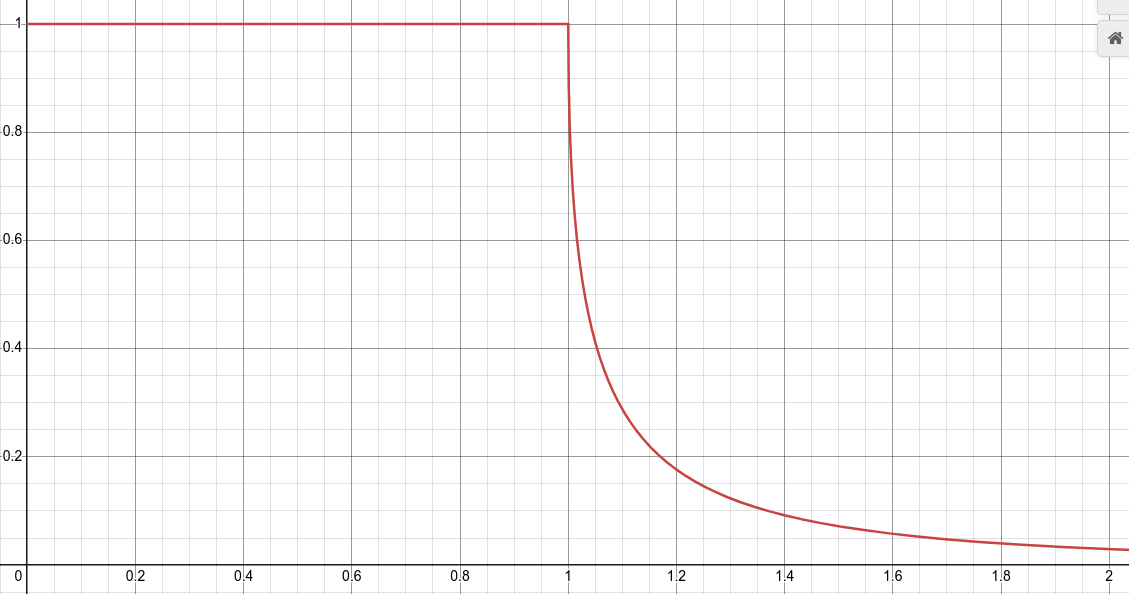
\includegraphics[width=.8\textwidth]{Figures/HW6-3a}
            \caption{Plot of Reflection Coefficient as a Function of Incident Energy}
            \label{fig:1}
          \end{figure}

          \begin{figure}[H]
            \centering
            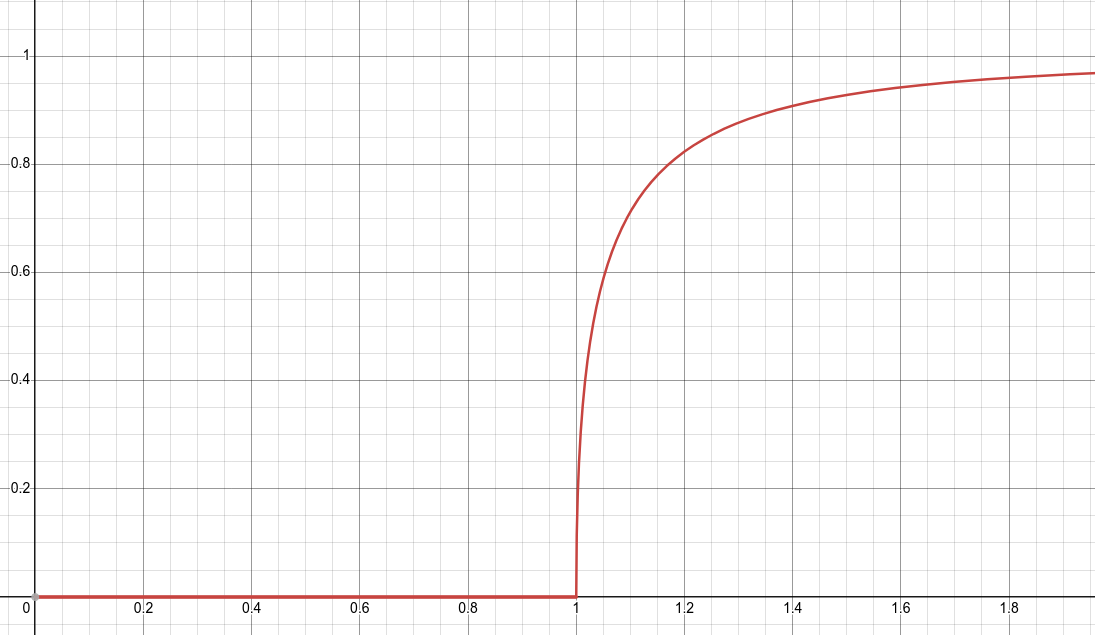
\includegraphics[width=.8\textwidth]{Figures/HW6-3b}
            \caption{Plot of Transmission Coefficient as a Function of Incident Energy}
            \label{fig:2}
          \end{figure}

          We may see that the reflection is unity and transmission is zero until the boundary is crossed. Then, the reflection decreases in a manner inversely proportional to the incident energy.

    \end{enumerate}

\end{enumerate}

\end{document}

